Il lavoro di questo tirocinio riguarda un progetto di Intecs SpA. L'azienda ha sviluppato un sistema di certificazione della posizione basato su tecnologia GNSS/SDR\footnote{Il GNSS/SDR è un software open source che si occupa di tutta l'elaborazione del segnale digitale, eseguendo l'acquisizione del segnale e il tracciamento dei segnali satellitari disponibili, decodificando il messaggio di navigazione e calcolando i dati necessari agli algoritmi di posizionamento per individuare la posizione.}. Lo scopo è stato quello di integrare la tecnologia di Algorand\footnote{Algorand è una blockchain incentrata sulla scalabilità e la decentralizzazione.} all’interno del dispositivo mobile che certifica la posizione, in modo che la certificazione venga realizzata direttamente su blockchain.

\section{Perché certificare la posizione?}
La certificazione della posizione è un problema fondamentale, visto che i sistemi che utilizzano strumenti di tipo GNSS (Global Navigation Satellite System)\footnote{L'acronimo GNSS (Global Navigation Satellite Systems) indica in modo generale i sistemi satellitari di posizionamento come il GPS (Stati Uniti) o GALILEO (Comunità Europea).} per rilevare la propria posizione, possono essere violati utilizzando una tecnica che prende il nome di spoofing. Quando un ricevitore raccoglie un segnale di navigazione da un satellite, non ha modo di confermare se il segnale sia effettivamente proveniente da quel satellite. Questa vulnerabilità può portare ad attuare delle tecniche di spoofing, ovvero di entità malintenzionate che utilizzano falsi segnali per fuorviare gli utenti sulla loro posizione effettiva [vedi figura \ref{fig: spoofing }]. Questo servizio di certificazione della posizione sviluppato da Intecs SpA offre un modo per prevenire tale attacco\cite{spoofing}.
\begin{figure}[h]
\centering
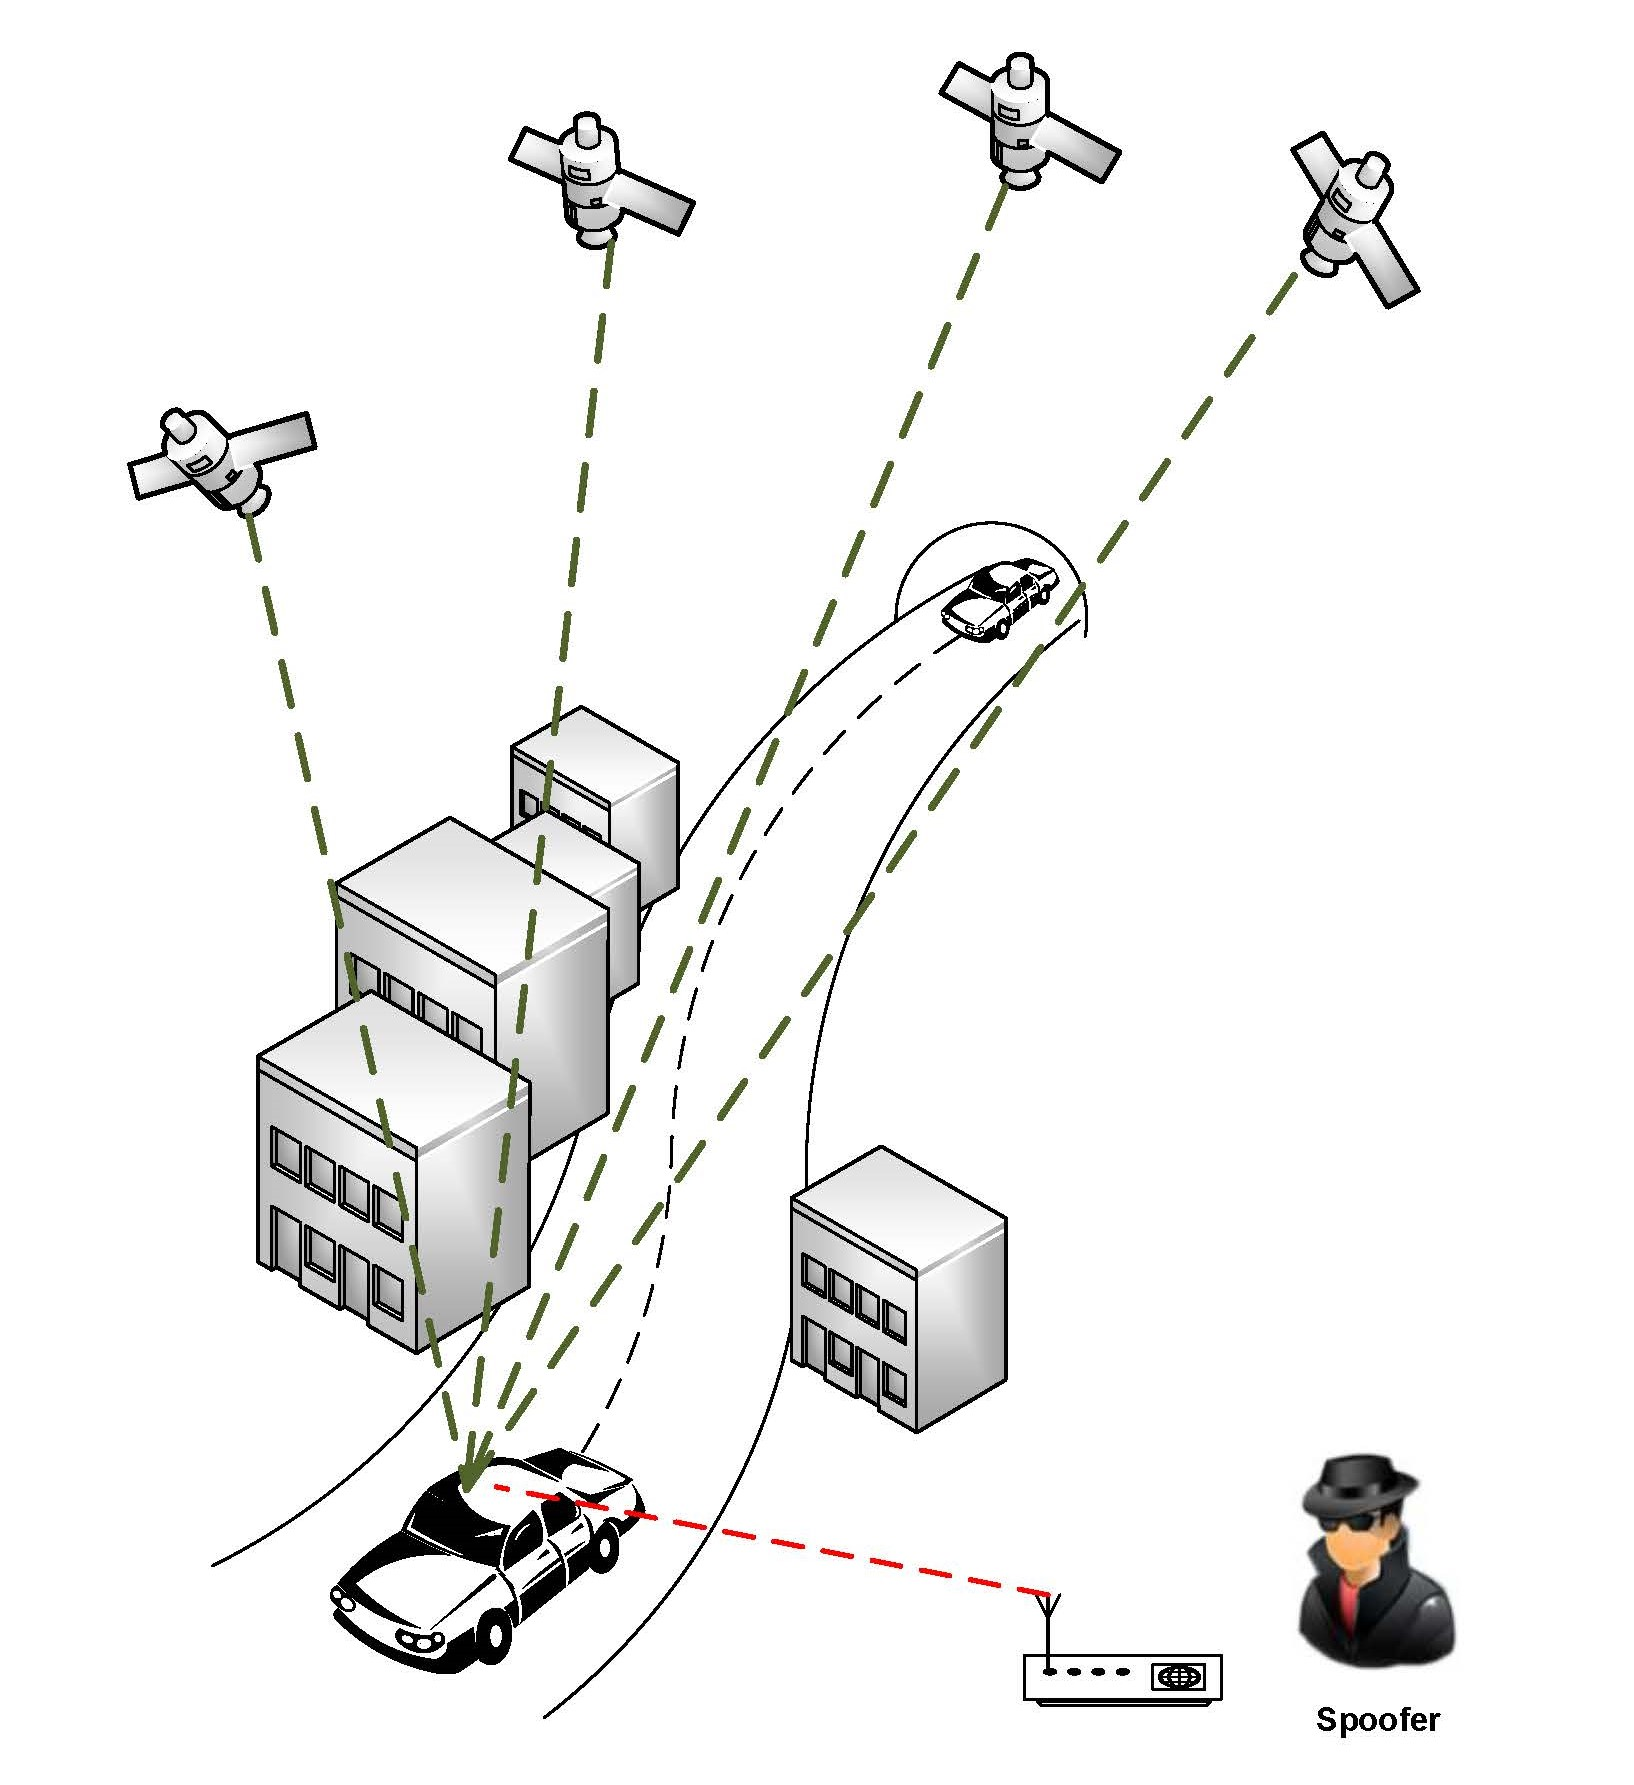
\includegraphics[scale=0.4]{images/Satnav_spoofing.jpg}
\caption{Un esempio di spoofing}
\label{fig: spoofing }
\end{figure}
Lo spoofing ad esempio, è stato dimostrato un mezzo in grado di forzare i droni o reindirizzare le navi, mentre alcuni luoghi ad alta sicurezza, come i confini internazionali interrotti, sono diventati noti per i segnali di spoofing che impediscono l'uso affidabile del navigatore satellitare nelle loro vicinanze. 

\subsection{Problemi dei sistemi GNSS}
Entriamo più nel dettaglio dei problemi di spoofing dei sistemi GNSS analizzando questa particolare tecnica. Considereremo da qui in avanti come sistema di posizionamento di riferimento il sistema di posizionamento Galileo\footnote{Il sistema di posizionamento Galileo è un sistema di posizionamento e navigazione satellitare civile, sviluppato in Europa come alternativa al GPS.}, visto che viene utilizzato da Intecs SpA per il loro sistema di certificazione della posizione. Informiamo il lettore che queste criticità si presentano anche negli altri sistemi di posizionamento come il GPS (Global Positioning System)\footnote{Il GPS (Global Positioning System) è un sistema di posizionamento e navigazione satellitare militare statunitense.}. Per individuare la posizione in cui ci troviamo si sfrutta un dispositivo di localizzazione che non fa altro che rimanere in ascolto dei segnali inviati dai satelliti e calcolare la distanza che intercorre tra sé e quest'ultimi, considerando il tempo di ricezione. Per effettuare un calcolo della posizione è necessario collegarsi ad almeno quattro satelliti, la cui posizione nello spazio è nota con precisione. Sfruttando i dati appena ottenuti è possibile calcolare l’intersezione delle quattro sfere immaginarie ed individuare la posizione del ricevitore. Spesso queste sfere si intersecheranno in parte invece che incontrarsi in un punto univoco e quindi il ricevitore calcolerà la posizione matematicamente più probabile. E' importante notare che il segnale dei satelliti catturato in una certa area è esattamente lo stesso di quello catturato nel raggio di alcune centinaia di km. Questo perché i satelliti si trovano distanti circa 23222 km dalla terra ed essendo posizionati molto in alto, coprono un'area molto estesa. Quello che cambia è il tempo con cui si riceverà il segnale dai satelliti trovandosi in due punti differenti. Un malintenzionato potrebbe catturare il segnale alla posizione A e ritrasmetterlo al dispositivo che si trova in posizione B accertandosi di essere in grado di oscurare il segnale dei satelliti in orbita. Un altro esempio a cui applicare questa tecnica di spoofing è con i pescherecci. Tipicamente hanno delle zone interdette dove non possono navigare e sono collegati ad un dispositivo GNSS per rilevare la posizione in tempo reale. Si può anche in questo caso sfruttare un escamotage: servirsi di un dispositivo che inganna il sistema che registra il segnale GNSS, facendogli registrare il segnale del sistema predisposto dall'attaccante invece del vero segnale acquisito dai satelliti.

\section{Che cos'è la Blockchain?}
La blockchain \cite{blockchain} (letteralmente "catena di blocchi") è una struttura dati condivisa e "immutabile". È definita come un registro digitale le cui transazioni sono raggruppate in "blocchi", concatenati in ordine cronologico, e la cui integrità è garantita dall'uso della crittografia. Il suo contenuto una volta scritto, non è più modificabile né eliminabile, a meno di non invalidare l'intera struttura. Le tecnologie basate su blockchain sono incluse nella più ampia famiglia dei Distributed Ledger, ossia sistemi che si basano su un registro distribuito, che può essere letto e modificato da più nodi di una rete. Non è richiesto che i nodi coinvolti conoscano l'identità reciproca o si fidino l'uno dell'altro perché, per garantire la coerenza tra le varie copie, l'aggiunta di un nuovo blocco è globalmente regolata da un protocollo di consenso eseguito da tutti i nodi. Una volta autorizzata l'aggiunta del nuovo blocco, ogni nodo aggiorna la propria copia privata. La natura stessa della struttura dati garantisce l'impossibilità di una sua manipolazione futura. Le caratteristiche che accomunano i sistemi sviluppati con le tecnologie blockchain e Distributed Ledger sono: digitalizzazione dei dati, decentralizzazione, tracciabilità dei trasferimenti, trasparenza/verificabilità, immutabilità del registro e programmabilità dei trasferimenti. Grazie a tali caratteristiche, la blockchain è considerata pertanto un'alternativa in termini di sicurezza, affidabilità, trasparenza e costi, alle banche dati e ai registri gestiti in maniera centralizzata da autorità riconosciute e regolamentate (pubbliche amministrazioni, banche, assicurazioni, intermediari di pagamento, ecc.).

% \subsection{Implementazione di una semplice Blockchain con Python}
% Diamo un'occhiata a una semplice implementazione di una blockchain in Python\footnote{Python è un linguaggio di programmazione dinamico orientato agli oggetti utilizzabile per molti tipi di sviluppo software.}. Innanzitutto, definiamo una funzione che chiamiamo bhash che, dato il timestamp e i dettagli (una stringa o un altro oggetto serializzabile) di una nuova transazione insieme all'hash della transazione precedente, calcola un nuovo hash utilizzando l'algoritmo SHA1:
% \begin{pythoncode}
% import hashlib, json, time

% def bhash (timestamp, details, prev_hash):
%     #la funzione dumps converte un oggetto Python in una stringa JSON
%     token = json.dumps([timestamp, details, prev_hash])
%     return hashlib.sha1(token).hexdigest())
% \end{pythoncode}
% Si noti che abbiamo usato il serializzatore json per combinare gli elementi insieme in una stringa che poi passiamo alla funzione hash SHA1 hash. La nostra scelta di serializzare in json è un dettaglio di implementazione e non l'unico modo per raggiungere l'obiettivo.
% Successivamente creiamo una classe Blockchain per incapsulare un elenco di blocchi:
% \begin{pythoncode}
% class Blockchain(object):
%     def __init__ (self, details='new-chain'):
%         self.blocks = [(time.time(), details, "")]
%     def record (self ,details, timestamp=None):
%         timestamp = timestamp or time.time()
%         #estraggo il campo hash dall'ultimo elemento della lista
%         prev_hash = self.blocks[-1][2]
%         new_hash = bhash(timestamp, details, prev_hash)
%         self.blocks.append((timestamp, details, new_hash))
% \end{pythoncode}
% La classe ha un costruttore, "init", che crea un elenco di blocchi e memorizza il primo blocco nell'elenco. Questo primo blocco contiene un timestamp iniziale e dettagli ma nessun hash. Nel caso di un bitcoin, questo memorizzerebbe informazioni sulla scoperta di una nuova unità e del suo proprietario.
% La classe ha anche un secondo metodo, "record", che, dati i dettagli di una nuova transazione e un timestamp opzionale (altrimenti calcolato automaticamente), li memorizza in un nuovo blocco. Questo viene fatto recuperando l'hash del blocco precedente da self.blocks [-1] [2] chiamando la funzione bhash e aggiungendo la tripla (timestamp, dettagli, new\_hash) all'elenco dei blocchi.
% Usiamo la nostra classe Blockchain creandone un'istanza, che chiamiamo "bc", e registriamo le transazioni rappresentate come stringhe autodescrittive:
% \begin{pythoncode}
% bc = Blockchain('A found 1 euro')
% bc.record('A gives 1 euro to B')
% bc.record('B gives 1 euro to C')
% bc.record('C gives 1 euro to D')
% \end{pythoncode}
% Quindi possiamo stampare i blocchi della blockchain con il comando seguente:
% \begin{pythoncode}
% print bc.blocks
% #output
% [(1495941516.704196, 'A found 1 euro', ""],
% (1495941516.704201, 'A gives 1 euro to B', 'a75a9227f...'),
% (1495941516.704277, 'B gives 1 euro to C', 'ca911be27...'),
% (1495941516.704290, 'C gives 1 euro to D', 'cb462885e...')]
% \end{pythoncode}
% L'ultimo hash è 'cb462885e...'. Affinché questa tecnologia funzioni, dobbiamo assicurarci di trasmettere l'ultimo hash e che ci siano alcune copie dell'intera blockchain memorizzate da parti diverse. Le parti in questo contesto sono i nodi di calcolo della rete peer-to-peer incaricati di registrare e archiviare le transazioni. Si tratta di un problema di rete che esula dall'ambito di questo articolo.
% È anche importante che ogni parte possa verificare l'integrità della blockchain. Questo può essere fatto facilmente utilizzando la funzione seguente:
% \begin{pythoncode}
% def verify (blockchain):
%     prev = blockchain.blocks[0]
%     for block in blockchain.blocks[1:]:
%         new_hash = bhash(block[0], block[1], prev[2])
%         if block[2] != new_hash: return False
%         prev = block
%     return True
% \end{pythoncode}
% Nel codice sopra, ripetiamo tutti i blocchi a partire dal secondo, ricalcoliamo ogni hash e poi lo confrontiamo con quello memorizzato in block[2]. Se il codice trova un hash che non corrisponde, restituisce False altrimenti restituisce True. Possiamo chiamare questo codice sulla nostra blockchain con:
% \begin{pythoncode}
% print verify(bc)
% #output
% True
% \end{pythoncode}
% Da un punto di vista tecnologico, c'è molto di più di questo nella rete Bitcoin. Esistono algoritmi per la distribuzione dei dati, per la sincronizzazione dei nodi, per l'archiviazione e l'interrogazione efficienti, per la risoluzione dei conflitti e così via, ma la tecnologia blockchain è al centro di esso\cite{8024092}.

\subsection{Blockchain nel progetto di tirocinio}
Per rendere più sicuro il sistema già esistente di certificazione della posizione, è stata utilizzata la tecnologia di Algorand \cite{algorand} attraverso l'introduzione di uno smart contract\footnote{Gli smart contract sono contratti che, una volta distribuiti, sono richiamabili in remoto da qualsiasi nodo nella blockchain di Algorand. Proprio come qualsiasi altro contratto, regola i termini e le condizioni di un accordo tra le parti.}, che ha reso possibile una maggiore sicurezza della comunicazione tra i componenti principali. Per quel che riguarda la sua creazione ed eliminazione, è stato deciso di concedere interamente ad Intecs SpA la possibilità di svolgere queste due operazioni. Sono anche state effettuate delle scelte implementative per impedire che lo smart contract non fosse in nessun modo modificato o eliminato da terzi. L'implementazione di questa procedura ha richiesto la creazione di un account Algorand ad uso esclusivo dell'azienda. Il lavoro di miglioramento del sistema di certificazione è stato svolto con l'obiettivo di conservare l'architettura del progetto di partenza.

\section{Breve riassunto dei capitoli successivi}
Nel capitolo \ref{2.statoarte} descriveremo i vari meccanismi di consenso delle diverse blockchain, della blockchain di Algorand e daremo un'introduzione al linguaggio PyTeal con cui vengono sviluppati gli smart contract. I meccanismi di consenso sono dei protocolli eseguiti all'interno di una rete distribuita e servono per validare le transazioni che sono state effettuate, ma possono servire anche per penalizzare chi decide di commettere irregolarità o chi non rispetta queste regole. La Proof of Work (PoW) e la Proof of Stake (PoS) sono i due algoritmi di consenso più famosi nel settore. Il primo utilizzato da Bitcoin, si basa sulla risoluzione di problemi matematici particolarmente complessi al fine di trovarne una soluzione chiamata "nonce"\footnote{Nonce è l’acronimo di “number only used once“, ovvero numero utilizzato una sola volta. Si riferisce al numero che un miner deve scoprire per poter risolvere un blocco nella blockchain.}. Il PoS, utilizzato da criptovalute come Solana e Cardano è un meccanismo di consenso in cui i validators garantiscono la validità delle operazioni effettuate impegnando una quota delle proprie criptovalute (dette "stake"). Algorand utilizza invece una versione diversa del PoS chiamata Pure Proof of Stake che sfrutta un protocollo di accordo bizantino per raggiungere il consenso tra gli utenti sulla prossima serie di transazioni. Vedremo anche i tool di sviluppo per Algorand, le operazioni richieste per collegarsi alla blockchain per ricercare informazioni e come scrivere direttamente su quest’ultima. Tramite Algod\footnote{Algod è uno strumento fornito da Algorand che approfondiremo nel capitolo \ref{2.statoarte}.} è possibile eseguire transazioni sulla blockchain mentre per supportare la ricerca si utilizza l'Indexer. Uno strumento rapido per creare e configurare un ambiente di sviluppo Algorand con Algod e Indexer prende il nome di Algorand Sandbox.

Daremo nel capitolo \ref{3.progetto iniziale} una descrizione del sistema di certificazione della posizione realizzato da Intecs SpA e introdurremo il sistema di posizionamento satellitare Galileo\cite{de2001galileo} per descrivere il suo funzionamento. Il progetto di partenza utilizza principalmente tre componenti: sistema centrale, sistema mobile e stazione di riferimento. Il sistema mobile e la stazione di riferimento acquisiscono nel solito istante, ogni 120 secondi, segnali cioè sequenze di bit dai satelliti Galileo in orbita sopra di loro. Per semplicità chiameremo l'insieme di questi segnali acquisiti da un solo dispositivo (sistema mobile o stazione di riferimento) "snapshot". Entrambe le componenti, ovvero il sistema mobile e la stazione di riferimento inviano lo snapshot catturato al sistema centrale che procederà con il confronto dei due snapshot per verificare la loro equivalenza.

Nel capitolo \ref{4.integriamo la blockchain} introdurremo il sistema degli smart contract, programmi che vengono archiviati sulla blockchain che possono generare transazioni di pagamenti, asset e possono anche memorizzare valori sulla blockchain. Sono in definitiva dei contratti che, una volta implementati, sono richiamabili in remoto. Per rendere più sicuro il sistema di certificazione della posizione già esistente è stato introdotto uno smart contract per far sì che alcune operazioni fossero più sicure e i dati di posizione immutabili.

Nel capitolo \ref{5.cli e intecs} daremo modo al lettore di capire come poter comunicare con il sistema di certificazione realizzato, introducendo due programmi fondamentali implementati con un'interfaccia a linea di comando: Cli e Intecs. Entrambi sono implementati con lo scopo di semplificare le varie operazioni (come il settaggio di parametri o la creazione ed eliminazione dello smart contract). Il programma Cli è univoco per ogni sistema mobile e nella prima versione (cli v1) rappresenta uno strumento per interfacciarsi al sistema mobile, poterlo interrogare e richiedere informazioni sugli snapshot ricevuti da quest'ultimo. Nella versione 2 (cli v2) il programma comunica direttamente con la blockchain di Algorand attraverso l'Indexer\footnote{Per ricercare informazioni nella blockchain di Algorand si fa uso di uno strumento chiamato Indexer V2. Lo scopo principale di questo indicizzatore è fornire un'interfaccia API REST di chiamate API per supportare la ricerca in Algorand Blockchain.} per estrarre informazioni dal campo nota di una particolare transazione che vedremo in seguito. 

Nel capitolo \ref{6.simulazione del progetto} mostriamo i vari step per poter avviare correttamente il progetto su un calcolatore\footnote{Il progetto è stato implementato e testato su sistema operativo Windows 10}. 

Infine, nel capitolo conclusivo (capitolo \ref{7.conclusioni}) mostriamo alcune implementazioni alternative rispetto al progetto realizzato e le features che non sono state realizzate per la mancanza di tempo a disposizione, che porterebbero però ad un maggior livello di sicurezza. Un'implementazione alternativa, analizzata solo concettualmente, che va nella direzione della filosofia di decentralizzazione che è intrinseca nella blockchain è quella di sfruttare una tecnologia decentralizzata anche per la memorizzazione dei dati. Nel progetto implementato, il sistema centrale archivia i file zip e JSON ricevuti dal sistema mobile e dalla stazione di riferimento internamente. Per evitare che questi file possano andare persi ed introdurre quindi una ridondanza, una soluzione sarebbe potuta essere quella di memorizzarli su IPFS\footnote{IPFS, acronimo di InterPlanetary File System, è file system decentralizzato, implementato con una rete peer-to-peer. Si tratta di un sistema per l'archiviazione e la condivisione di dati.}, un file system decentralizzato.